\chapter{Cornerstone models: Conjugate families}\label{chap4}

\section{Solutions of Exercises}\label{sec1}
\begin{enumerate}[leftmargin=*]
\item Write in the canonical form the distribution of the Bernoulli example, and find the mean and variance of the sufficient statistic.

\textbf{Answer}

Given $p({\bf{y}}|\theta)=(1-\theta)^N\exp\left\{\sum_{i=1}^N y_i\log\left(\frac{\theta}{1-\theta}\right)\right\}$ where $\eta=\log\frac{\theta}{1+\theta}$ which implies $\theta=\frac{\exp(\eta)}{1-\exp(\eta)}$, then $p({\bf{y}}|\theta)=\exp\left\{\sum_{i=1}^N y_i\eta-N\log(1+\exp(\eta))\right\}$. Thus $B(\eta)=N\log(1+\exp(\eta))$, $\nabla(B(\eta))=N\frac{\exp(\eta)}{1+\exp(\eta)}=N\theta$ and $\nabla^2(B(\eta))=N\left\{\frac{\exp(\eta)(1+\exp(\eta))}{(1+\exp(\eta))^2}-\frac{\exp(\eta)\exp(\eta)}{(1+\exp(\eta))^2}\right\}=N\theta(1-\theta)$. 



\item Given a random sample $\mathbf{y}=[y_1,y_2,\dots,y_N]^{\top}$ from $N$ \textit{binomial experiments} each having known size $n_i$ and same unknown probability $\theta$. Show that $p(\mathbf{y}|\theta)$ is in the exponential family, and find the posterior distribution, the marginal likelihood and the predictive distribution of the binomial-beta model assuming the number of trials is known.

\textbf{Answer}

The density function is 
\begin{align*}
p({\bf{y}}|\theta)&=\prod_{i=1}^N{n_i \choose y_i}\theta^{y_i}(1-\theta)^{n_i-y_i}\\
&=\prod_{i=1}^N{n_i \choose y_i}\theta^{\sum_{i=1}^Ny_i}(1-\theta)^{\sum_{i=1}^N n_i-\sum_{i=1}^N y_i}\\
&=\prod_{i=1}^N{n_i \choose y_i}\exp\left\{\sum_{i=1}^N y_i\log\left(\frac{\theta}{1-\theta}\right)+\sum_{i=1}^N n_i\log(1-\theta)\right\}\\
&=\prod_{i=1}^N{n_i \choose y_i}(1-\theta)^{\sum_{i=1}^N n_i}\exp\left\{\sum_{i=1}^N y_i\log\left(\frac{\theta}{1-\theta}\right)\right\},
\end{align*}
 
Observe that $\sum_{i=1}^N n_i$ is the total sample size of Bernoulli experiments. 

Using Theorem 1 in Chapter 4, the prior distribution is \begin{align*}\pi(\theta)&\propto(1-\theta)^{B_0}\exp\left\{a_0\log\left(\frac{\theta}{1-\theta}\right)\right\}\\
	&=\theta^{a_0}(1-\theta)^{B_0-a_0}\\
	&=\theta^{\alpha_0-1}(1-\theta)^{\beta_0-1},
\end{align*}

where $\alpha_0=a_0+1$ and $\beta_0=B_0-a_0+1$. This is the kernel of a beta distribution. Thus, the posterior distribution is

\begin{align*}
	\pi(\theta|{\bf{y}})&\propto \theta^{\alpha_0-1}(1-\theta)^{\beta_0-1} \times \theta^{\sum_{i=1}^Ny_i}(1-\theta)^{\sum_{i=1}^N n_i-\sum_{i=1}^N y_i}\\
	&=\theta^{\alpha_0+\sum_{i=1}^Ny_i - 1}(1-\theta)^{\beta_0 + \sum_{i=1}^N n_i-\sum_{i=1}^N y_i - 1}\\
	&=\theta^{\alpha_n-1}(1-\theta)^{\beta_n-1},  
\end{align*}

where $\alpha_n = \alpha_0+\sum_{i=1}^Ny_i$ and $\beta_n=\beta_0 + \sum_{i=1}^N n_i-\sum_{i=1}^N y_i$.

The marginal likelihood is

\begin{align*}
	p({\bf{y}})&=\int_0^1 \frac{\theta^{\alpha_0-1}(1-\theta)^{\beta_0-1}}{B(\alpha_0,\beta_0)}\times \prod_{i=1}^N{n_i \choose y_i}\theta^{\sum_{i=1}^Ny_i}(1-\theta)^{\sum_{i=1}^N n_i-\sum_{i=1}^N y_i} d\theta\\
	&=\frac{ \prod_{i=1}^N{n_i \choose y_i}}{B(\alpha_0,\beta_0)}\int_0^1 \theta^{\alpha_0+\sum_{i=1}^Ny_i-1}(1-\theta)^{}\beta_0\sum_{i=1}^N n_i-\sum_{i=1}^N y_i-1 d\theta\\
	&=\frac{ \prod_{i=1}^N{n_i \choose y_i}B(\alpha_n,\beta_n)}{B(\alpha_0,\beta_0)}. 
\end{align*}

The third line due to having the kernel of a Beta distribution.

Finally, the predictive distribution is

\begin{align*}
	p(Y_0|{\bf{y}})&=\int_0^1 {n_{y_0} \choose y_0} \theta^{y_0}(1-\theta)^{n_{y_0}-y_0}\frac{\theta^{\alpha_n-1}(1-\theta)^{\beta_n-1}}{B(\alpha_n,\beta_n)}d\theta\\
	&=\frac{{n_{y_0} \choose y_0}}{B(\alpha_n,\beta_n)}\int_0^1  \theta^{\alpha_n+y_0-1}(1-\theta)^{\beta_n+n_{y_0}-y_0-1}d\theta\\
	&={n_{y_0} \choose y_0}\frac{B(\alpha_n+y_0,\beta_n+n_{y_0}-y_0)}{B(\alpha_n,\beta_n)},
\end{align*}

where $n_{y_0}$ is the known size associated with $y_0$, and the last line due to having the kernel of a beta distribution. The predictive is a \textit{beta-binomial distribution}.

\item Given a random sample $\mathbf{y}=[y_1,y_2,\dots,y_N]^{\top}$ from a \textit{exponential distribution}. Show that $p(\mathbf{y}|\lambda)$ is in the exponential family, and find the posterior distribution, marginal likelihood and predictive distribution of the exponential-gamma model.

\textbf{Answer}

We see that the exponential distribution belongs to the exponential family as $p({\bf{y}}|\lambda)=\prod_{i=1}^N\lambda\exp(-\lambda y_i)=\lambda^N\exp(-\lambda\sum_{i=1}^N y_i)$.

Using the gamma distribution in the rate parametrization, we see that $\pi(\lambda|{\bf{y}})\propto \lambda^{\alpha_0-1}\exp(-\lambda\beta_0)\times \lambda^N\exp(-\lambda\sum_{i=1}^N y_i)=\lambda^{\alpha_0+N-1}\exp(-\lambda(\beta_0+\sum_{i=1}^N y_i))$. This is the kernel of a gamma distribution, that is, $\lambda|{\bf{y}}\sim G(\alpha_n,\beta_n)$ where $\alpha_n=\alpha_0+N$ and $\beta_n=\beta_0+\sum_{i=1}^N y_i$.

The marginal likelihood is

\begin{align*}
	p({\bf{y}})&=\int_0^{\infty}\lambda^N \exp\left\{-\lambda\sum_{i=1}^N\right\}\lambda^{\alpha_0-1}\exp\left\{-\beta_0\lambda\right\}\frac{\beta_0^{\alpha_0}}{\Gamma(\alpha_0)}d\lambda\\
	&=\frac{\beta_0^{\alpha_0}}{\Gamma(\alpha_0)}\int_0^{\infty}\lambda^{\alpha_0+N-1} \exp\left\{-\lambda\left(\beta_0+\sum_{i=1}^N\right)\right\}d\lambda\\
	&=\frac{\beta_0^{\alpha_0}\Gamma(\alpha_n)}{\Gamma(\alpha_0)\beta_n^{\alpha_n}}.
\end{align*} 

Finally, the predictive distribution is

\begin{align*}
	p(Y_0|{\bf{y}})&=\int_0^{\infty}\lambda \exp\left\{-\lambda y_0\right\}\lambda^{\alpha_n-1}\exp\left\{-\beta_n\lambda\right\}\frac{\beta_n^{\alpha_n}}{\Gamma(\alpha_n)}d\lambda\\
	&=\frac{\beta_n^{\alpha_n}}{\Gamma(\alpha_n)}\int_0^{\infty}\lambda^{\alpha_n+1-1}\exp\left\{-\lambda(\beta_n+y_0)\right\}d\lambda\\
	&=\frac{\beta_n^{\alpha_n}}{\Gamma(\alpha_n)}\times \frac{\Gamma(\alpha_n+1)}{(\beta_n+y_0)^{\alpha_n+1}}\\
	&=\frac{\alpha_n\beta_n^{\alpha_n}}{(\beta_n+y_0)^{\alpha_n+1}}.
\end{align*} 

This is a \textit{Lomax distribution}.

\item Given $\mathbf{y}\sim N_N(\bm{\mu},\bm{\Sigma})$, that is, a \textit{multivariate normal distribution} show that $p(\mathbf{y}|\bm{\mu},\bm{\Sigma})$ is in the exponential family.

\textbf{Answer} 

\begin{align}
	p(\mathbf{y}|\bm{\mu},\bm{\Sigma})&= (2\pi)^{-N/2}|\bm{\Sigma}|^{-1/2}\exp\left\{-\frac{1}{2}\left(\mathbf{y}-\bm{\mu}\right)^{\top}\bm{\Sigma}^{-1}\left(\mathbf{y}-\bm{\mu}\right)\right\}\nonumber\\
	&= (2\pi)^{-N/2}\exp\left\{-\frac{1}{2}\left(\mathbf{y}^{\top}\bm{\Sigma}^{-1}\mathbf{y}-2\mathbf{y}^{\top}\bm{\Sigma}^{-1}\bm{\mu}+\bm{\mu}^{\top}\bm{\Sigma}^{-1}\bm{\mu}+\log(|\mathbf{\Sigma}|)\right)\right\}\nonumber\\
	&= (2\pi)^{-N/2}\exp\left\{-\frac{1}{2}\left(tr\left\{\mathbf{y}^{\top}\bm{\Sigma}^{-1}\mathbf{y}\right\}-2\mathbf{y}^{\top}\bm{\Sigma}^{-1}\bm{\mu}+\bm{\mu}^{\top}\bm{\Sigma}^{-1}\bm{\mu}+\log(|\mathbf{\Sigma}|)\right)\right\}\nonumber\\
	&= (2\pi)^{-N/2}\exp\left\{-\frac{1}{2}\left(vec\left(\mathbf{y}\mathbf{y}^{\top}\right)^{\top}vec\left(\bm{\Sigma}^{-1}\right)-2\mathbf{y}^{\top}\bm{\Sigma}^{-1}\bm{\mu}+\bm{\mu}^{\top}\bm{\Sigma}^{-1}\bm{\mu}+\log(|\mathbf{\Sigma}|)\right)\right\} \nonumber, 	
\end{align}

where $tr$ and $vec$ are the trace and vectorization operators, respectively. 

Then, $h(\mathbf{y})=(2\pi)^{-N/2}$, $\eta(\bm{\mu},\bm{\Sigma})=\left[\bm{\Sigma}^{-1}\bm{\mu} \ \ vec\left(\bm{\Sigma}^{-1}\right)\right]$, $T(\mathbf{y})=\left[\mathbf{y} \ \ -\frac{1}{2}vec(\mathbf{y}\mathbf{y}^{\top})\right]$ and $C(\bm{\mu},\bm{\Sigma})=\exp\left\{-\frac{1}{2N}\left(\bm{\mu}^{\top}\bm{\Sigma}^{-1}\bm{\mu}+\log(|\mathbf{\Sigma}|)\right)\right\}$.
	
\item Find the marginal likelihood in the normal/inverse-Wishart model.

\textbf{Answer}

\begin{align*}
	p({\bf{Y}})=&\int_{\mathcal{R}^p}\int_{\mathcal{S}}(2\pi)^{-pN/2}|\mathbf{\Sigma}|^{-N/2}\exp\left\{-\frac{1}{2}tr[({\bf{S}}+N(\bm{\mu}-\hat{\bm{\mu}})(\bm{\mu}-\hat{\bm{\mu}})^{\top})\mathbf{\Sigma}^{-1}]\right\}\\
	&\times (2\pi)^{-p/2}\beta_0^{p/2}|\mathbf{\Sigma}|^{-1/2}\exp\left\{-\frac{\beta_0}{2}tr[(\bm{\mu}-\bm{\mu}_0)(\bm{\mu}-\bm{\mu}_0)^{\top}\mathbf{\Sigma}^{-1}]\right\}\\
	&\times |\mathbf{\Sigma}|^{-(\alpha_0+p+1)/2}\frac{2^{-\alpha_0p/2}|\mathbf{\Psi}_0|^{\alpha_0/2}}{\Gamma_p(\alpha_0/2)}\exp\left\{-\frac{1}{2}tr(\mathbf{\Psi}_0\mathbf{\Sigma}^{-1})\right\}d\mathbf{\Sigma} d\bm{\mu}\\
	&=\frac{(2\pi)^{-frac{1}{2}(pN+p)}|\mathbf{\Psi}_0|^{\alpha_0/2}\beta_0^{p/2}2^{-\alpha_0p/2}}{\Gamma_p(\alpha_0/2)}\int_{\mathcal{R}^p}\int_{\mathcal{S}} |\mathbf{\Sigma}|^{-\frac{1}{2}(N+1+\alpha_0+p+1)}\\
	&\times \exp\left\{-\frac{1}{2}tr[({\bf{S}}+N(\bm{\mu}-\hat{\bm{\mu}})(\bm{\mu}-\hat{\bm{\mu}})^{\top}+\beta_0(\bm{\mu}-\bm{\mu}_0)(\bm{\mu}-\bm{\mu}_0)^{\top}+\mathbf{\Psi}_0)\mathbf{\Sigma}^{-1}]\right\}d\mathbf{\Sigma} d\bm{\mu}.
\end{align*}

We have in the integral the kernel of an Inverse-Wishart distribution, then

\begin{align*}
p({\bf{Y}})	&=\frac{\Gamma_p\left(\frac{N+1+\alpha_0}{2}\right)|\mathbf{\Psi}_0|^{\alpha_0/2}\beta_0^{p/2}}{\Gamma_p(\alpha_0/2)\pi^{p(N+1)/2}}\\
	&\times\int_{\mathcal{R}^p} |{\bf{S}}+\mathbf{\Psi}_0+(N+\beta_0)(\bm{\mu}-\bm{\mu}_n)(\bm{\mu}-\bm{\mu}_n)^{\top}\\
	&+N\beta_0/(N+\beta_0)(\hat{\bm{\mu}}-\bm{\mu}_0)(\hat{\bm{\mu}}-\bm{\mu}_0)^{\top}| d\bm{\mu}\\
	&=\frac{\Gamma_p\left(\frac{N+1+\alpha_0}{2}\right)|\mathbf{\Psi}_0|^{\alpha_0/2}\beta_0^{p/2}}{\Gamma_p(\alpha_0/2)\pi^{p(N+1)/2}}\\
	&\times\int_{\mathcal{R}^p} |\mathbf{\Psi}_n||1+\beta_n(\bm{\mu}-\bm{\mu}_n)\mathbf{\Psi}_n^{-1}(\bm{\mu}-\bm{\mu}_n)^{\top}|^{-\frac{1}{2}(\alpha_n+1)} d\bm{\mu}\\
	&=\frac{\Gamma_p\left(\frac{\alpha_n+1}{2}\right)|\mathbf{\Psi}_0|^{\alpha_0/2}\beta_0^{p/2}}{\Gamma_p(\alpha_0/2)\pi^{p(N+1)/2}}|\mathbf{\Psi}_n|^{-\frac{1}{2}(\alpha_n+1)}\\
	&\times\int_{\mathcal{R}^p} [1+\beta_n(\bm{\mu}-\bm{\mu}_n)^{\top}\mathbf{\Psi}_n^{-1}(\bm{\mu}-\bm{\mu}_n)]^{-\frac{1}{2}(\alpha_n+1)} d\bm{\mu}.
\end{align*} 

The last equality uses the definition of $\mathbf{\Psi}_n$, $\beta_n$ and $\alpha_n$, and the Sylvester's determinant theorem. Observe that we have the kernel of a multivariate t distribution \cite{murphy2007conjugate}. Then,

\begin{align*}
	p({\bf{Y}})	&=\frac{\Gamma_p\left(\frac{\alpha_n+1}{2}\right)|\mathbf{\Psi}_0|^{\alpha_0/2}\beta_0^{p/2}}{\Gamma_p(\alpha_0/2)\pi^{p(N+1)/2}}|\mathbf{\Psi}_n|^{-\frac{1}{2}(\alpha_n+1)}\\
	&\times\int_{\mathcal{R}^p} \left[ 1+\frac{1}{\alpha_n+1-p}(\bm{\mu}-\bm{\mu}_n)^{\top}\left(\frac{\mathbf{\Psi}_n}{\beta_n(\alpha_n+1-p)}\right)^{-1}(\bm{\mu}-\bm{\mu}_n)\right]^{-\frac{1}{2}(\alpha_n+1-p+p)} d\bm{\mu}\\
	&=\frac{\Gamma_p\left(\frac{\alpha_n+1}{2}\right)\Gamma_p\left(\frac{\alpha_n+1-p}{2}\right)|\mathbf{\Psi}_0|^{\alpha_0/2}\beta_0^{p/2}(\alpha_n+1-p)^{p/2}\pi^{p/2}|\mathbf{\Psi}_n|^{-\frac{1}{2}(\alpha_n+1)}}{\Gamma_p(\alpha_0/2)\pi^{p(N+1)/2}\Gamma_p\left(\frac{\alpha_n+1-p+p}{2}\right)\left(\frac{\mathbf{\Psi}_n}{\alpha_n+1-p}\right)^{-1/2}}\\
	&=\frac{\Gamma_p\left(\frac{v_n}{2}\right)}{\Gamma_p\left(\frac{\alpha_0}{2}\right)}\frac{|\mathbf{\Psi}_0|^{\alpha_0/2}}{|\mathbf{\Psi}_n|^{\alpha_n/2}}\left(\frac{\beta_0}{\beta_n}\right)^{p/2}(2\pi)^{-Np/2},
\end{align*}

where $v_n=\alpha_n+1-p$.


\item Find the posterior predictive distribution in the normal/inverse-Wishart model, and show that ${\bf{Y}}_0|{\bf{Y}}\sim T_{N_0,M}(\alpha_n-M+1,{\bf{X}}_0{\bf{B}}_n,{\bf{I}}_{N_0}+{\bf{X}}_0{\bf{V}}_n{\bf{X}}_0^{\top},{\bf{\Psi}}_n)$ in the multivariate regression linear model.

\textbf{Answer}

\begin{align*}
	p({\bf{Y}}_0|{\bf{Y}})&\propto\int_{\mathcal{R}^p}\int_{\mathcal{S}}|\mathbf{\Sigma}|^{-1/2}\exp\left\{-\frac{1}{2}tr[({\bf{y}}_0-\bm{\mu})({\bf{y}}_0-\bm{\mu})^{\top}\mathbf{\Sigma}^{-1}]\right\}\\
	&\times |\mathbf{\Sigma}|^{-1/2}\exp\left\{-\frac{\beta_n}{2}tr[(\bm{\mu}-\bm{\mu}_n)(\bm{\mu}-\bm{\mu}_n)^{\top}\mathbf{\Sigma}^{-1}]\right\}\\
	&\times |\mathbf{\Sigma}|^{-(\alpha_n+p+1)/2}\exp\left\{-\frac{1}{2}tr(\mathbf{\Psi}_n \mathbf{\Sigma}^{-1})\right\}d\mathbf{\Sigma} d\bm{\mu}\\
	&\propto\int_{\mathcal{R}^p}|({\bf{y}}_0-\bm{\mu})({\bf{y}}_0-\bm{\mu})^{\top}+(\bm{\mu}-\bm{\mu}_n)(\bm{\mu}-\bm{\mu}_n)^{\top}+\mathbf{\Psi}_n|^{-(\alpha_n+2)/2}d\bm{\mu}.
\end{align*}

The last equality uses that there is the kernel of an Inverse Wishart distribution.

Taking into account that

{\scriptsize{
\begin{align*}
	({\bf{y}}_0-\bm{\mu})({\bf{y}}_0-\bm{\mu})^{\top}+(\bm{\mu}-\bm{\mu}_n)(\bm{\mu}-\bm{\mu}_n)^{\top} & = (1+\beta_n)\left(\bm{\mu}-\frac{({\bf{y}}_0+\beta_n\bm{\mu}_n)}{1+\beta_n}\right)\left(\bm{\mu}-\frac{({\bf{y}}_0+\beta_n\bm{\mu}_n)}{1+\beta_n}\right)^{\top}\\
	&+\frac{\beta_n}{1+\beta_n}({\bf{y}}_0-\bm{\mu}_n)({\bf{y}}_0-\bm{\mu}_n)^{\top}.
\end{align*}
}}

Then,
{\scriptsize{
\begin{align*}
	p({\bf{Y}}_0|{\bf{Y}})&\propto\int_{\mathcal{R}^p}|({\bf{y}}_0-\bm{\mu})({\bf{y}}_0-\bm{\mu})^{\top}+(\bm{\mu}-\bm{\mu}_n)(\bm{\mu}-\bm{\mu}_n)^{\top}+\mathbf{\Psi}_n|^{-(\alpha_n+2)/2}d\bm{\mu}\\
	&=\int_{\mathcal{R}^p}\left\vert(1+\beta_n)\left(\bm{\mu}-\frac{({\bf{y}}_0+\beta_n\bm{\mu}_n)}{1+\beta_n}\right)\left(\bm{\mu}-\frac{({\bf{y}}_0+\beta_n\bm{\mu}_n)}{1+\beta_n}\right)^{\top}\right.\\
	&\left.+\frac{\beta_n}{1+\beta_n}({\bf{y}}_0-\bm{\mu}_n)({\bf{y}}_0-\bm{\mu}_n)^{\top}+\mathbf{\Psi}_n\right\vert^{-(\alpha_n+2)/2}d\bm{\mu}\\
	&=\int_{\mathcal{R}^p}\left[\left\vert\underbrace{\mathbf{\Psi}_n+\frac{\beta_n}{1+\beta_n}({\bf{y}}_0-\bm{\mu}_n)({\bf{y}}_0-\bm{\mu}_n)^{\top}}_{\mathbf{\Lambda}_n}\right\vert\right.\\
	&\left.\left\vert 1+(1+\beta_n)\left(\bm{\mu}-\frac{({\bf{y}}_0+\beta_n\bm{\mu}_n)}{1+\beta_n}\right)^{\top}\frac{1}{\alpha_n+2-p}\left(\frac{\mathbf{\Lambda}_n}{\alpha_n+2-p}\right)^{-1}\left(\bm{\mu}-\frac{({\bf{y}}_0+\beta_n\bm{\mu}_n)}{1+\beta_n}\right)\right\vert\right]^{-(\alpha_n+2-p+p)/2}d\bm{\mu}\\
	&\propto \left\vert\mathbf{\Psi}_n+\frac{\beta_n}{1+\beta_n}({\bf{y}}_0-\bm{\mu}_n)({\bf{y}}_0-\bm{\mu}_n)^{\top}\right\vert^{-(\alpha_n+2)/2}\\
	&\times \left\vert\mathbf{\Psi}_n+\frac{\beta_n}{1+\beta_n}({\bf{y}}_0-\bm{\mu}_n)({\bf{y}}_0-\bm{\mu}_n)^{\top}\right\vert^{1/2}\\
	&=\left\vert\mathbf{\Psi}_n+\frac{\beta_n}{1+\beta_n}({\bf{y}}_0-\bm{\mu}_n)({\bf{y}}_0-\bm{\mu}_n)^{\top}\right\vert^{-(\alpha_n+1)/2}\\
	&\propto \left[1+({\bf{y}}_0-\bm{\mu}_n)^{\top}\frac{1}{\alpha_n+1-p}\left(\frac{\mathbf{\Psi}_n(1+\beta_n)}{(\alpha_n+1-p)\beta_n}\right)^{-1}({\bf{y}}_0-\bm{\mu}_n)\right]^{-(\alpha_n+1-p+p)}. 
\end{align*} 
}}

The second equality and last line use the Sylvester's determinant theorem, and the second equality uses that there is the kernel of a multivariate t distribution.

Then, we have that the predictive distribution is a multivariate t distribution centered at $\bm{\mu}_n$, $\alpha_n+1-p$ degrees of freedom, and scale matrix $\frac{\mathbf{\Psi}_n(1+\beta_n)}{(\alpha_n+1-p)\beta_n}$.

To show the second statement, let's start by the definition of the predictive density to show that ${\bf{Y}}_0|{\bf{Y}}\sim T_{N_0,M}(\alpha_n-M+1,{\bf{X}}_0{\bf{B}}_n,{\bf{I}}_{N_0}+{\bf{X}}_0{\bf{V}}_n{\bf{X}}_0^{\top},{\bf{\Psi}}_n)$.

\begin{align*}
	\pi({\bf{Y}}_0|{\bf{Y}})&\propto\int_{\mathcal{S}}\int_{\mathcal{B}}\left\{ |{\bf{\Sigma}}|^{-N_0/2}\exp\left\{-\frac{1}{2}tr[({\bf{Y}}_0-{\bf{X}}_0{\bf{B}})^{\top}({\bf{Y}}_0-{\bf{X}}_0{\bf{B}}){\bf{\Sigma}^{-1}}]\right\}\right.\\
	&\times |{\bf{\Sigma}}|^{-K/2}\exp\left\{-\frac{1}{2}tr[({\bf{B}}-{\bf{B}}_n)^{\top}{\bf{V}}_n^{-1}({\bf{B}}-{\bf{B}}_n){\bf{\Sigma}^{-1}}]\right\}\\
	&\times\left. |{\bf{\Sigma}}|^{-(\alpha_n+M+1)/2}\exp\left\{-\frac{1}{2}tr[{\bf{\Psi}}_n{\bf{\Sigma}^{-1}}]\right\}\right\}d{\bf{B}}d{\bf{\Sigma}}\\
	&=\int_{\mathcal{S}}\int_{\mathcal{B}}\left\{ |{\bf{\Sigma}}|^{-(N_0+K+\alpha_n+M+1)/2}\exp\left\{-\frac{1}{2}tr\left[\left(({\bf{Y}}_0-{\bf{X}}_0{\bf{B}})^{\top}({\bf{Y}}_0-{\bf{X}}_0{\bf{B}})\right.\right.\right.\right.\\
	&\left.\left.\left.\left.+({\bf{B}}-{\bf{B}}_n)^{\top}{\bf{V}}_n^{-1}({\bf{B}}-{\bf{B}}_n)+{\bf{\Psi}}_n\right){\bf{\Sigma}^{-1}}\right]\right\}\right\}d{\bf{B}}d{\bf{\Sigma}}.	 
\end{align*}

Setting ${\bf{M}}=({\bf{X}}_0^{\top}{\bf{X}}_0+{\bf{V}}_n^{-1})$, and ${\bf{B}}_{*}={\bf{M}}^{-1}({\bf{V}}_n{\bf{B}}_n+{\bf{X}}_0^{\top}{\bf{Y}}_0)$, we have that $({\bf{B}}-{\bf{B}}_*)^{\top}{\bf{M}}({\bf{B}}-{\bf{B}}_*)+{\bf{B}}_n^{\top}{\bf{V}}_n^{-1}{\bf{B}}_n+{\bf{Y}}_0^{\top}{\bf{Y}}_0-{\bf{B}}_*^{\top}{\bf{M}}{\bf{B}}_*=({\bf{Y}}_0-{\bf{X}}_0{\bf{B}})^{\top}({\bf{Y}}_0-{\bf{X}}_0{\bf{B}})+({\bf{B}}-{\bf{B}}_n)^{\top}{\bf{V}}_n^{-1}({\bf{B}}-{\bf{B}}_n)$. Then,

\begin{align*}
	\pi({\bf{Y}}_0|{\bf{Y}})&\propto \int_{\mathcal{S}}|{\bf{\Sigma}}|^{-(N_0+K+\alpha_n+M+1)/2}\\
	&\times \exp\left\{-\frac{1}{2}tr[({\bf{\Psi}}_n+{\bf{B}}_n^{\top}{\bf{V}}_n^{-1}{\bf{B}}_n+{\bf{Y}}_0^{\top}{\bf{Y}}_0-{\bf{B}}_*^{\top}{\bf{M}}{\bf{B}}_*){\bf{\Sigma}^{-1}}]\right\}\\
	&\times\int_{\mathcal{B}}\exp\left\{-\frac{1}{2}tr[({\bf{B}}-{\bf{B}}_*)^{\top}{\bf{M}}({\bf{B}}-{\bf{B}}_*){\bf{\Sigma}^{-1}}]\right\}d{\bf{B}}d{\bf{\Sigma}}.
\end{align*} 

The latter is the kernel of a matrix normal distribution, thus

\begin{align*}
	\pi({\bf{Y}}_0|{\bf{Y}})&\propto \int_{\mathcal{S}}|{\bf{\Sigma}}|^{-(N_0+\alpha_n+M+1)/2}\\
	&\times \exp\left\{-\frac{1}{2}tr[({\bf{\Psi}}_n+{\bf{B}}_n^{\top}{\bf{V}}_n^{-1}{\bf{B}}_n+{\bf{Y}}_0^{\top}{\bf{Y}}_0-{\bf{B}}_*^{\top}{\bf{M}}{\bf{B}}_*){\bf{\Sigma}^{-1}}]\right\}d{\bf{\Sigma}}\\
\end{align*}

This is the kernel of an inverse-Wishart distribution, then

\begin{align*}
	\pi({\bf{Y}}_0|{\bf{Y}})&\propto \left|{\bf{\Psi}}_n+{\bf{B}}_n^{\top}{\bf{V}}_n^{-1}{\bf{B}}_n+{\bf{Y}}_0^{\top}{\bf{Y}}_0-{\bf{B}}_*^{\top}{\bf{M}}{\bf{B}}_*\right|^{-(N_0+\alpha_n)/2}.
\end{align*} 

Setting ${\bf{C}}^{-1}={\bf{I}}_{N_0}+{\bf{X}}_0{\bf{V}}_n{\bf{X}}_0^{\top}$ such that ${\bf{C}}={\bf{I}}_{N_0}-{\bf{X}}_0({\bf{X}}_0^{\top}{\bf{X}}_0+{\bf{V}}_n^{-1})^{-1}{\bf{X}}_0^{\top}$ (see footnote 4 in Chapter 4), then ${\bf{B}}_n^{\top}{\bf{V}}_n^{-1}{\bf{B}}_n+{\bf{Y}}_0^{\top}{\bf{Y}}_0-{\bf{B}}_*^{\top}{\bf{M}}{\bf{B}}_*=({\bf{Y}}_0-{\bf{X}}_0{\bf{B}}_n)^{\top}{\bf{C}}({\bf{Y}}_0-{\bf{X}}_0{\bf{B}}_n)$. This is done following exactly same procedure as deducing the predictive distribution in the linear regression model in the book. Thus,
\begin{align*}
	\pi({\bf{Y}}_0|{\bf{Y}})&\propto \left|{\bf{\Psi}}_n+({\bf{Y}}_0-{\bf{X}}_0{\bf{B}}_n)^{\top}{\bf{C}}({\bf{Y}}_0-{\bf{X}}_0{\bf{B}}_n)\right|^{-(N_0+\alpha_n)/2}\\
	&\propto\left|{\bf{I}}_{N_0}+{\bf{C}}({\bf{Y}}_0-{\bf{X}}_0{\bf{B}}_n){\bf{\Psi}}^{-1}({\bf{Y}}_0-{\bf{X}}_0{\bf{B}}_n)^{\top}\right|^{-(\alpha_n+1-M+N_0+M-1)/2}.
\end{align*} 
The second proportionality follows from the Sylvester's theorem. Observe that this is the kernel of a matrix t distribution with $\alpha_n+1-M$ degrees of freedom, location ${\bf{X}}_0{\bf{B}}_n$ and scale matrices ${\bf{\Psi}}_n$ and ${\bf{C}}^{-1}={\bf{I}}_{N_0}+{\bf{X}}_0{\bf{V}}_n{\bf{X}}_0^{\top}$.     

\item Show that $\delta_n=\delta_0+({\bf{y}}-{\bf{X}}\hat{\bm{\beta}})^{\top}({\bf{y}}-{\bf{X}}\hat{\bm{\beta}})+(\hat{\bm{\beta}}-\bm{\beta}_0)^{\top}(({\bf{X}}^{\top}{\bf{X}})^{-1}+{\bf{B}}_0)^{-1}(\hat{\bm{\beta}}-\bm{\beta}_0)$ in the linear regression model, and that ${\bf{\Psi}}_{n}={\bf{\Psi}}_{0}+{\bf{S}}+(\hat{\bf{B}}-{\bf{B}}_{0})^{\top}{\bf{V}}_{n}(\hat{\bf{B}}-{\bf{B}}_{0})$ in the linear multivariate regression model. 

\textbf{Answer}

Taking into account that 
\begin{align*}
	\delta^* & = \delta_0 + {\bf{y}}^{\top}{\bf{y}} + \bm{\beta}_0^{\top}{\bf{B}}_0^{-1}\bm{\beta}_0 - \bm{\beta}_n^{\top}{\bf{B}}_n^{-1}\bm{\beta}_n \\
	& = \delta_0 + {\bf{y}}^{\top}{\bf{y}} + \bm{\beta}_0^{\top}{\bf{B}}_0^{-1}\bm{\beta}_0 -({\bf{B}}_0^{-1}\bm{\beta}_0 + {\bf{X}}^{\top}{\bf{X}}\hat{\bm{\beta}})^{\top}{\bf{B}}_n({\bf{B}}_0^{-1}\bm{\beta}_0 + {\bf{X}}^{\top}{\bf{X}}\hat{\bm{\beta}}) \\
	& = \delta_0 + {\bf{y}}^{\top}{\bf{y}} - \hat{\bm{\beta}}^{\top}{\bf{X}}^{\top}{\bf{X}}{\bf{B}}_n{\bf{X}}^{\top}{\bf{X}}\hat{\bm{\beta}} - 2\hat{\bm{\beta}}^{\top}{\bf{X}}^{\top}{\bf{X}}{\bf{B}}_n{\bf{B}}_0^{-1}\bm{\beta}_0 + \bm{\beta}_0^{\top}({\bf{B}}_0^{-1} - {\bf{B}}_0^{-1}{\bf{B}}_n{\bf{B}}_0^{-1})\bm{\beta}_0 \\
	&- \hat{\bm{\beta}}^{\top}{\bf{X}}^{\top}{\bf{X}}\hat{\bm{\beta}} + \hat{\bm{\beta}}^{\top}{\bf{X}}^{\top}{\bf{X}}\hat{\bm{\beta}} \\
	& = \delta_0 + {\bf{y}}^{\top}{\bf{y}} - \hat{\bm{\beta}}^{\top}{\bf{X}}^{\top}{\bf{X}}\hat{\bm{\beta}} + \hat{\bm{\beta}}^{\top}({\bf{X}}^{\top}{\bf{X}} - {\bf{X}}^{\top}{\bf{X}}{\bf{B}}_n{\bf{X}}^{\top}{\bf{X}})\hat{\bm{\beta}} \\
	& - 2\hat{\bm{\beta}}^{\top}{\bf{X}}^{\top}{\bf{X}}{\bf{B}}_n{\bf{B}}_0^{-1}\bm{\beta}_0 + \bm{\beta}_0^{\top}({\bf{B}}_0^{-1} - {\bf{B}}_0^{-1}{\bf{B}}_n{\bf{B}}_0^{-1})\bm{\beta}_0. 
\end{align*}

Observe that 
\begin{align*}
	({\bf{y}} - {\bf{X}}\hat{\bm{\beta}})^{\top}({\bf{y}} - {\bf{X}}\hat{\bm{\beta}}) & = {\bf{y}}^{\top}{\bf{y}} - 2\hat{\bm{\beta}}{\bf{X}}^{\top}{\bf{y}} + \hat{\bm{\beta}}^{\top}{\bf{X}}^{\top}{\bf{X}}\hat{\bm{\beta}}\\
	& = {\bf{y}}^{\top}{\bf{y}} - 2\hat{\bm{\beta}}^{\top}{\bf{X}}^{\top}({\bf{X}}\hat{\bm{\beta}}+\hat{\bm{\mu}}) + \hat{\bm{\beta}}^{\top}{\bf{X}}^{\top}{\bf{X}}\hat{\bm{\beta}}\\
	& = {\bf{y}}^{\top}{\bf{y}} - \hat{\bm{\beta}}^{\top}{\bf{X}}^{\top}{\bf{X}}\hat{\bm{\beta}},
\end{align*}
where ${\bf{y}}={\bf{X}}\hat{\bm{\beta}}+\hat{\bm{\mu}}$, and ${\bf{X}}^{\top}\hat{\bm{\mu}}=0$.

The following matrix identities are useful \cite{Smith1973}:
%\begin{equation}\label{eq:a}
%D + E & = E(E^{-1} + D^{-1})D
%\end{equation}

\begin{equation*}
	({\bf{D}} + {\bf{E}})^{-1} = {\bf{D}}^{-1} - {\bf{D}}^{-1}({\bf{D}}^{-1} + {\bf{E}}^{-1})^{-1}{\bf{D}}^{-1},
\end{equation*}
and
\begin{equation*}
	({\bf{D}} + {\bf{E}})^{-1} = {\bf{D}}^{-1}({\bf{E}}^{-1} + {\bf{D}}^{-1}){\bf{E}}^{-1}.
\end{equation*}

Using these identities,
\begin{align*}
	[({\bf{X}}^{\top}{\bf{X}})^{-1} + {\bf{B}}_0]^{-1} & = {\bf{X}}^{\top}{\bf{X}} - {\bf{X}}^{\top}{\bf{X}}({\bf{X}}^{\top}{\bf{X}} + {\bf{B}}_0^{-1})^{-1}{\bf{X}}^{\top}{\bf{X}} \\
	& = {\bf{B}}_0^{-1} - {\bf{B}}_0^{-1}({\bf{X}}^{\top}{\bf{X}} + {\bf{B}}_0^{-1})^{-1}{\bf{B}}_0^{-1}\\
	& = {\bf{X}}^{\top}{\bf{X}}({\bf{X}}^{\top}{\bf{X}} + {\bf{B}}_0^{-1})^{-1}{\bf{B}}_0^{-1}. 
\end{align*}
Then, 
\begin{align*}
	\delta^* & = \delta_0+ ({\bf{y}} - {\bf{X}}\hat{\bm{\beta}})^{\top}({\bf{y}} - {\bf{X}}\hat{\bm{\beta}}) + \hat{\bm{\beta}}^{\top}[({\bf{X}}^{\top}{\bf{X}})^{-1} + {\bf{B}}_0]^{-1}\hat{\bm{\beta}} \\
	& - 2\hat{\bm{\beta}}[({\bf{X}}^{\top}{\bf{X}})^{-1} + {\bf{B}}_0]^{-1}\bm{\beta}_0 + \bm{\beta}_0^{\top}[({\bf{X}}^{\top}{\bf{X}})^{-1} + {\bf{B}}_0]^{-1}\bm{\beta}_0\\
	& = \delta_0+ ({\bf{y}} - {\bf{X}}\hat{\bm{\beta}})^{\top}({\bf{y}} - {\bf{X}}\hat{\bm{\beta}})\\
	& + (\hat{\bm{\beta}} - \bm{\beta}_0)^{\top}[({\bf{X}}^{\top}{\bf{X}})^{-1} + {\bf{B}}_0]^{-1}(\hat{\bm{\beta}} - \bm{\beta}_0).
\end{align*}

In a similar way for the second part,

\begin{align*}
	({\bf{V}}_0+({\bf{X}}^{\top}{\bf{X}})^{-1})^{-1}&={\bf{V}}_0^{-1}-{\bf{V}}_0^{-1}({\bf{V}}_0^{-1}+{\bf{X}}^{\top}{\bf{X}})^{-1}{\bf{V}}_0^{-1}\\
	&={\bf{X}}^{\top}{\bf{X}}-{\bf{X}}^{\top}{\bf{X}}({\bf{V}}_0^{-1}+{\bf{X}}^{\top}{\bf{X}})^{-1}{\bf{X}}^{\top}{\bf{X}}\\
	&={\bf{X}}^{\top}{\bf{X}}(({\bf{X}}^{\top}{\bf{X}})^{-1}+{\bf{V}}_0)^{-1}{\bf{V}}_0^{-1},
\end{align*}

we use these results and some algebra to show that ${\bf{B}}_{0}^{\top}{\bf{V}}_{0}^{-1}{\bf{B}}_{0}+\widehat{\bf{B}}^{\top}{\bf{X}}^{\top}{\bf{X}}\widehat{\bf{B}}-{\bf{B}}_n^{\top}{\bf{V}}_n^{-1}{\bf{B}}_n=(\hat{\bf{B}}-{\bf{B}}_{0})^{\top}{\bf{V}}_{n}(\hat{\bf{B}}-{\bf{B}}_{0})$ taking into account that ${\bf{V}}_n = ({\bf{V}}_{0}^{-1}+{\bf{X}}^{\top}{\bf{X}})^{-1}$ and $\widehat{\bf{B}}= ({\bf{X}}^{\top}{\bf{X}})^{-1}{\bf{X}}^{\top}{\bf{Y}}$.


\item Show that in the linear regression model $\bm{\beta}_n^{\top}({\bf{B}}_n^{-1}-{\bf{B}}_n^{-1}{\bf{M}}^{-1}{\bf{B}}_n^{-1})\bm{\beta}_n=\bm{\beta}_{**}^{\top}{\bf{C}}\bm{\beta}_{**}$ and $\beta_{**}={\mathbf{X}}_0\beta_n$.

\textbf{Answer}

Taking into account that $({\bf{A}}+{\bf{B}})^{-1}={\bf{A}}^{-1}-{\bf{A}}^{-1}({\bf{A}}^{-1}+{\bf{B}}^{-1})^{-1}{\bf{A}}^{-1}$ \cite{Smith1973}, then we observe that $({\bf{B}}_n^{-1}-{\bf{B}}_n^{-1}{\bf{M}}^{-1}{\bf{B}}_n^{-1})=({\bf{B}}_n+({\bf{X}}_0^{\top}{\bf{X}}_0)^{-1})^{-1}$, where $({\bf{B}}_n+({\bf{X}}_0^{\top}{\bf{X}}_0)^{-1})^{-1}={\bf{X}}_0^{\top}{\bf{X}}_0-{\bf{X}}_0^{\top}{\bf{X}}_0({\bf{B}}_n^{-1}+{\bf{X}}_0^{\top}{\bf{X}}_0)^{-1}{\bf{X}}_0^{\top}{\bf{X}}_0={\bf{X}}_0^{\top}{\bf{X}}_0-{\bf{X}}_0^{\top}{\bf{X}}_0{\bf{M}}^{-1}{\bf{X}}_0^{\top}{\bf{X}}_0$, thus
\begin{align*}
	\bm{\beta}_n^{\top}({\bf{B}}_n^{-1}-{\bf{B}}_n^{-1}{\bf{M}}^{-1}{\bf{B}}_n^{-1})\bm{\beta}_n&=\bm{\beta}_n^{\top}({\bf{X}}_0^{\top}{\bf{X}}_0-{\bf{X}}_0^{\top}{\bf{X}}_0{\bf{M}}^{-1}{\bf{X}}_0^{\top}{\bf{X}}_0)\bm{\beta}_n\\
	&=\bm{\beta}_n^{\top}{\bf{X}}_0^{\top}({\bf{I}}_{N_0}-{\bf{X}}_0{\bf{M}}^{-1}{\bf{X}}_0^{\top}){\bf{X}}_0\bm{\beta}_n\\
	&=\bm{\beta}_n^{\top}{\bf{X}}_0^{\top}{\bf{C}}{\bf{X}}_0\bm{\beta}_n\\
	&=\bm{\beta}_{**}^{\top}{\bf{C}}\bm{\beta}_{**}.
\end{align*}

Let's show that $\bm{\beta}_{**}={\mathbf{X}}_0\bm{\beta}_n$,

\begin{align*}
	\bm{\beta}_{**}&={\bf{C}}^{-1}{\bf{X}}_0{\bf{M}}^{-1}{\bf{B}}_n^{-1}\bm{\beta}_n\\
	&=({\bf{I}}_{N_0}+{\bf{X}}_0{\bf{B}}_n{\bf{X}}_0^{\top}){\bf{X}}_0{\bf{M}}^{-1}{\bf{B}}_n^{-1}\bm{\beta}_n\\
	&=({\bf{I}}_{N_0}+{\bf{X}}_0{\bf{B}}_n{\bf{X}}_0^{\top}){\bf{X}}_0({\bf{B}}_n-{\bf{B}}_n(({\bf{X}}_0^{\top}{\bf{X}}_0)^{-1}+{\bf{B}}_n)^{-1}{\bf{B}}_n){\bf{B}}_n^{-1}\bm{\beta}_n\\
	&=({\bf{I}}_{N_0}+{\bf{X}}_0{\bf{B}}_n{\bf{X}}_0^{\top})({\bf{X}}_0\bm{\beta}_n-{\bf{X}}_0{\bf{B}}_n(({\bf{X}}_0^{\top}{\bf{X}}_0)^{-1}+{\bf{B}}_n)^{-1}\bm{\beta}_n)\\
	&={\bf{X}}_0\bm{\beta}_n-{\bf{X}}_0{\bf{B}}_n(({\bf{X}}_0^{\top}{\bf{X}}_0)^{-1}+{\bf{B}}_n)^{-1}\bm{\beta}_n+{\bf{X}}_0{\bf{B}}_n{\bf{X}}_0^{\top}{\bf{X}}_0\bm{\beta}_n\\
	&-{\bf{X}}_0{\bf{B}}_n{\bf{X}}_0^{\top}{\bf{X}}_0{\bf{B}}_n(({\bf{X}}_0^{\top}{\bf{X}}_0)^{-1}+{\bf{B}}_n)^{-1}\bm{\beta}_n\\
	&={\bf{X}}_0\bm{\beta}_n-{\bf{X}}_0{\bf{B}}_n[(({\bf{X}}_0^{\top}{\bf{X}}_0)^{-1}+{\bf{B}}_n)^{-1}-{\bf{X}}_0^{\top}{\bf{X}}_0+{\bf{X}}_0^{\top}{\bf{X}}_0{\bf{B}}_n(({\bf{X}}_0^{\top}{\bf{X}}_0)^{-1}+{\bf{B}}_n)^{-1}]\bm{\beta}_n.
\end{align*}

Using that $({\bf{A}}+{\bf{B}})^{-1}={\bf{A}}^{-1}-{\bf{A}}^{-1}{\bf{B}}({\bf{A}}+{\bf{B}})^{-1}$, we observe that the expression in brackets is equal to ${\bf{0}}$, then we have the result.

\item Show that $({\bf{Y}}-{\bf{X}}{\bf{B}})^{\top}({\bf{Y}}-{\bf{X}}{\bf{B}})={\bf{S}}+({\bf{B}}-\widehat{\bf{B}})^{\top}{\bf{X}}^{\top}{\bf{X}}({\bf{B}}-\widehat{\bf{B}})$ where ${\bf{S}}= ({\bf{Y}}-{\bf{X}}\widehat{\bf{B}})^{\top}({\bf{Y}}-{\bf{X}}\widehat{\bf{B}})$, $\widehat{\bf{B}}= ({\bf{X}}^{\top}{\bf{X}})^{-1}{\bf{X}}^{\top}{\bf{Y}}$ in the multivariate regression model.

\textbf{Answer}
\begin{align*}
	({\bf{Y}}-{\bf{X}}{\bf{B}})^{\top}({\bf{Y}}-{\bf{X}}{\bf{B}})&=({\bf{Y}}-{\bf{X}}\hat{{\bf{B}}}+{\bf{X}}\hat{{\bf{B}}}-{\bf{X}}{\bf{B}})^{\top}({\bf{Y}}-{\bf{X}}\hat{{\bf{B}}}+{\bf{X}}\hat{{\bf{B}}}-{\bf{X}}{\bf{B}})\\
	&=({\bf{Y}}-{\bf{X}}\hat{{\bf{B}}})^{\top}({\bf{Y}}-{\bf{X}}\hat{{\bf{B}}})+2({\bf{Y}}-{\bf{X}}\hat{{\bf{B}}})^{\top}({\bf{X}}\hat{{\bf{B}}}-{\bf{X}}{\bf{B}})\\
	&+({\bf{X}}{\bf{B}}-{\bf{X}}\hat{{\bf{B}}})^{\top}({\bf{X}}{\bf{B}}-{\bf{X}}\hat{{\bf{B}}})\\
	&={\bf{S}}+({\bf{B}}-\hat{{\bf{B}}})^{\top}{\bf{X}}^{\top}{\bf{X}}({\bf{B}}-\hat{{\bf{B}}}),
\end{align*}

given that $({\bf{Y}}-{\bf{X}}\hat{{\bf{B}}})^{\top}({\bf{X}}\hat{{\bf{B}}}-{\bf{X}}{\bf{B}})=\hat{\bf{U}}^{\top}{\bf{X}}(\hat{{\bf{B}}}-{\bf{B}})$, using that $\hat{{\bf{B}}}=({\bf{X}}^{\top}{\bf{X}})^{-1}{\bf{X}}^{\top}{\bf{Y}}$ which implies ${\bf{X}}^{\top}{\bf{X}}\hat{{\bf{B}}}={\bf{X}}^{\top}{\bf{Y}}={\bf{X}}^{\top}{\bf{X}}\hat{\bf{B}}+{\bf{X}}^{\top}\hat{\bf{U}}$, then ${\bf{X}}^{\top}\hat{\bf{U}}={\bf{0}}$.

	\item \textbf{What is the probability that the Sun will rise tomorrow?}

This is the most famous Richard Price's example developed in the Appendix of the Bayes' theorem paper \cite{bayes1763lii}. Here, we implicitly use \textit{Laplace's Rule of Succession} to solve this question. In particular, if we were a priori uncertain about the probability the Sun will rise on a specified day, we can assume a prior uniform distribution over (0,1), that is, a beta (1,1) distribution. Then, what is the probability that the Sun will rise tomorrow?

\textbf{Answer}

This exercise is an application of the Bernoulli-beta model. Thus, the likelihood is given by a binomial distribution where the probability of success is $\theta$, $p(\mathbf{y}|\theta)\propto\theta^{\sum_{i=1}^N y_i}(1-\theta)^{N-\sum_{i=1}^N y_i}$. In addition, the prior distribution is beta, that is, $\pi(\theta)\propto \theta^{\alpha_0-1}(1-\theta)^{\beta_0-1}$, where $\alpha_0=\beta_0=1$. Then, the predictive distribution that the sun will rise tomorrow is  $p(Y_0=1|\mathbf{y})=\frac{1+S}{2+N}$, where $S=\sum_{i=1}^N y_i$ is the number of successes (the Sun rise). $\frac{1+S}{2+N}$ is known as the \textit{Laplace's Rule of Succession} that was introduced by Laplace in the 18$^{th}$ century in the course of treating the sunrise problem.  

	\item Using information from Public Policy Polling in September 27th-28th for the 2016 presidential five-way race in USA, there are 411, 373 and 149 sampled people supporting Hillary Clinton, Donald Trump and other, respectively. 

\begin{itemize}
	\item Find the posterior probability of the percentage difference of people supporting Hillary versus Trump according to this data using a non-informative prior, that is, $\alpha_0=[1 \ 1 \ 1]$ in the multinomial-Dirichlet model. What is the probability of having more supporters of Hillary vs Trump?
	
	\item What is the probability that sampling one hundred independent individuals 44, 40 and 16 support Hillary, Trump and other, respectively?  
\end{itemize}

\textbf{Answer}

\begin{tcolorbox}[enhanced,width=4.67in,center upper,
	fontupper=\large\bfseries,drop shadow southwest,sharp corners]
	\textit{R code. Multinomial-Dirichlet model: Polling 2016 USA presidential race}
\begin{VF}
\begin{lstlisting}[language=R]
set.seed(010101)
# Multinomial-Dirichlet example: 
# Polling 2016 USA presidential race
y <- c(411, 373, 149) 
# Clinton, Trump, Other
# Public Policy Polling September 27-28, 
# 2016 five-way race
alpha0 <- rep(1, 3)
# Hyperparameters: non-informative distribution
alphan <- alpha0 + y 
S <- 100000 
# Sample draws of posterior
thetas <- MCMCpack::rdirichlet(S, alphan)
colnames(thetas) <- c("Clinton", "Trump", "Other")
head(thetas)
       Clinton     Trump     Other
[1,] 0.4211346 0.4188607 0.1600046
[2,] 0.4244207 0.4224523 0.1531270
[3,] 0.4349268 0.3843953 0.1806779
[4,] 0.4533499 0.4005530 0.1460972
[5,] 0.4381799 0.3968502 0.1649699
[6,] 0.4436852 0.3971321 0.1591827
dif <- thetas[,1] - thetas[,2]
# Difference of shares Hillary vs Trump
data <- data.frame(dif)
names(data) <- c("Difference")
library(ggplot2)
p <- ggplot(data) +  
	geom_histogram(aes(x = Difference), binwidth = 0.01) +
	geom_vline(xintercept=0.0, lwd=1, colour="red") + 
	ggtitle("Percentage difference Clinton vs Trump 2016 presidential race") + xlab("Percentage Difference") + ylab("")
difmcmc <- coda::mcmc(dif)
# Declaring a MCMC object
summary(difmcmc)

Iterations = 1:1e+05
Thinning interval = 1 
Number of chains = 1 
Sample size per chain = 1e+05 

1. Empirical mean and standard deviation for each 
variable, plus standard error of the mean:

Mean             SD       Naive SE Time-series SE 
4.062e-02      2.996e-02      9.474e-05      9.474e-05 
2. Quantiles for each variable:

2.5%      25%      50%      75%    97.5% 
-0.01817  0.02033  0.04058  0.06089  0.09923 
CW <- mean(difmcmc>0)
CW
0.91339
\end{lstlisting}
\end{VF}
\end{tcolorbox} 

\begin{figure}[!h]
	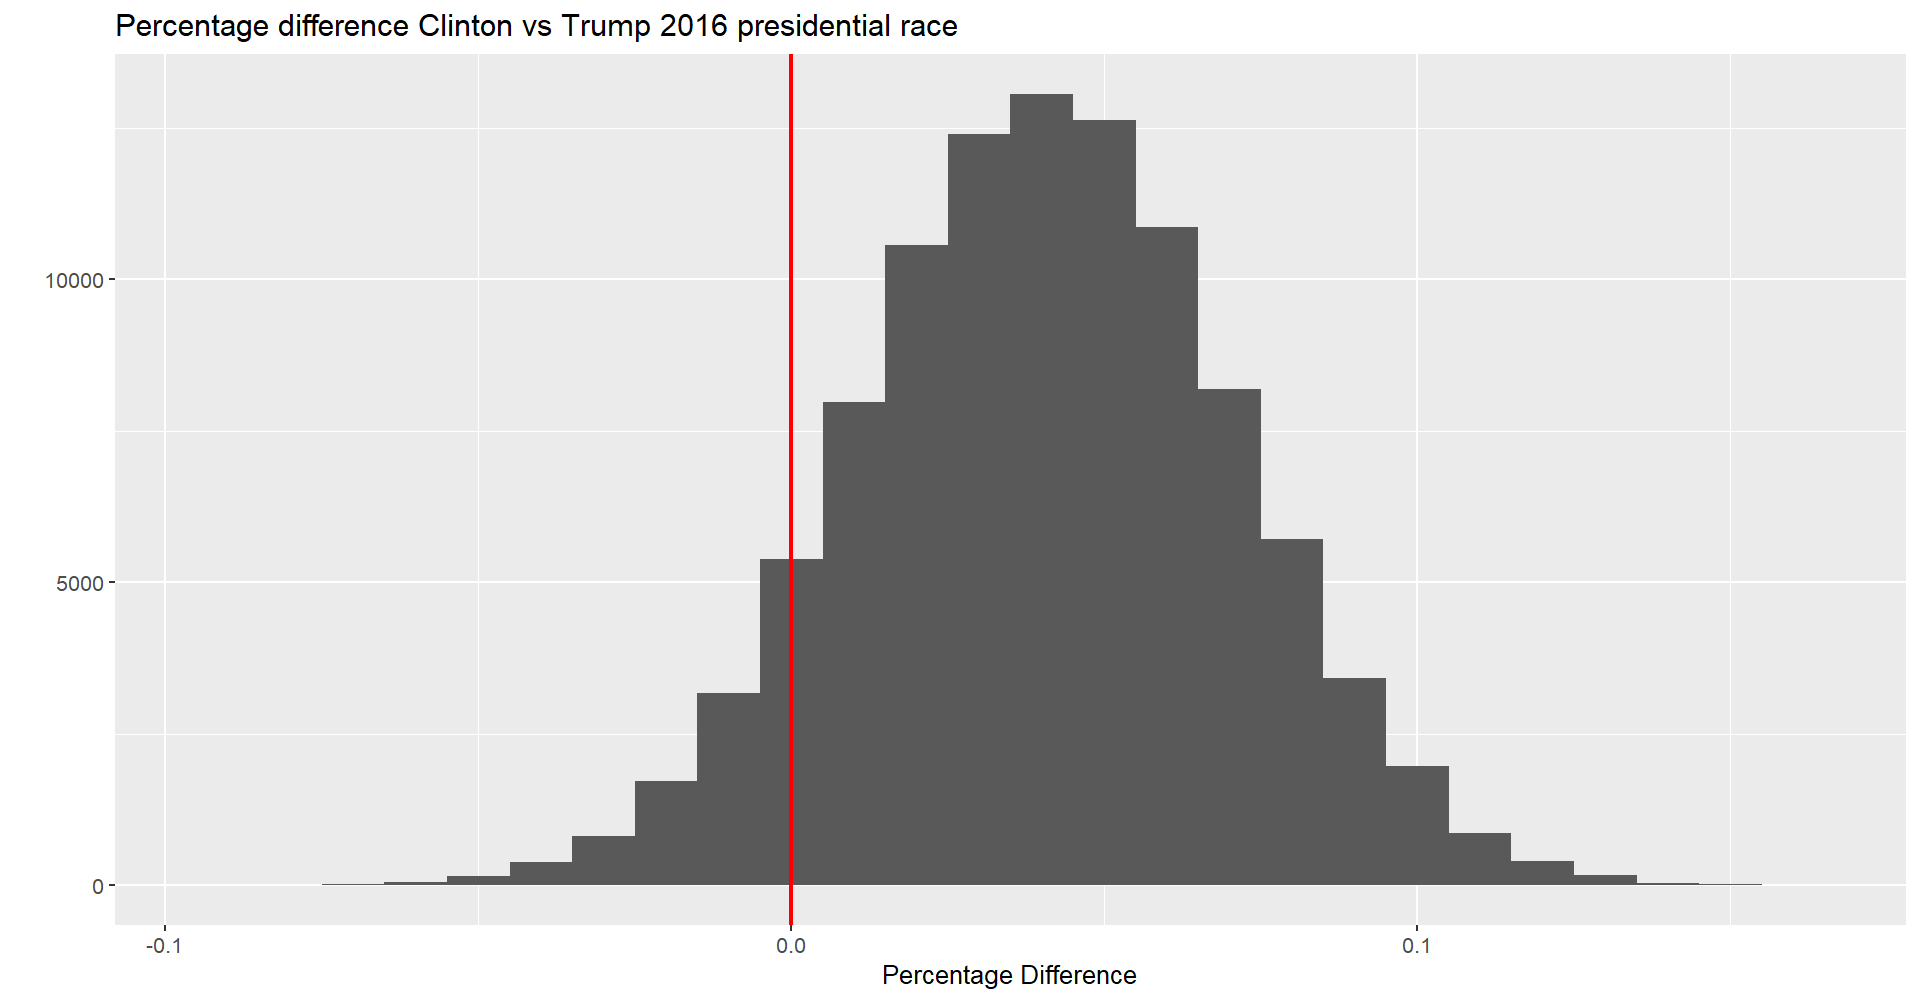
\includegraphics[width=340pt, height=200pt]{Chapters/chapter4/figures/hiillaryVStrump.png}
	%%\centerline{\epsfig{/Chapters/chapter1/figures/cat.eps,width=.8\textheight,height=.4\textwidth}}
	\caption[List of figure caption goes here]{Percentage difference: Hillary Clinton vs Donald Trump, five-way race.}\label{fig41}
\end{figure}

There is a 95\% probability that the percentage difference between Hillary and Trump according to this poll is (-1.8\%, 9.9\%). The probability of Hillary having more supporters is 91.3\%


\begin{tcolorbox}[enhanced,width=4.67in,center upper,
	fontupper=\large\bfseries,drop shadow southwest,sharp corners]
	\textit{R code. Multinomial-Dirichlet model: Polling 2016 USA presidential race}
\begin{VF}
\begin{lstlisting}[language=R]
# Predictive distribution by simulation
y0 <- c(44, 40, 16)
Pred <- apply(thetas, 1, function(p) {rmultinom(1, size = sum(y0), prob = p)})
sum(sapply(1:S, function(s) {sum(Pred[,s] == y0) == 3}))/S
0.00825
# Predictive distribution by analytical expression
PredY0 <- function(y0){
	n <- sum(y0)
	Res1 <- sum(sapply(1:length(y), function(l){lgamma(alphan[l]+y0[l]) - lgamma(alphan[l])-lfactorial(y0[l])}))
	Res <- lfactorial(n)+lgamma(sum(alphan))-lgamma(sum(alphan)+n) + Res1
	return(exp(Res))
}
PredY0(y0)
0.00850         
\end{lstlisting}
\end{VF}
\end{tcolorbox} 

The probability that from one hundred random selected people 44 support Hillary, 40 support Trump and 16 support other candidate is 0.85\%.

\item \textbf{Math test example continues}

You have a random sample of math scores of size $N=50$ from a normal distribution, $Y_i\sim \mathcal{N}(\mu, \sigma)$. The sample mean and variance are equal to $102$ and $10$, respectively. Using the normal-normal/inverse-gamma model where $\mu_0=100$, $\beta_0=1$, $\alpha_0=\delta_0=0.001$

\begin{itemize}
	\item Get 95\% confidence and credible intervals for $\mu$.
	\item What is the posterior probability that $\mu > 103$?  
\end{itemize}  

{\textbf{Answer}}

\begin{tcolorbox}[enhanced,width=4.67in,center upper,
	fontupper=\large\bfseries,drop shadow southwest,sharp corners]
	\textit{R code. Math test example continues}
\begin{VF}
\begin{lstlisting}[language=R]
set.seed(010101)
N <- 50
# Sample size
muhat <- 102
# Sample mean
sig2hat <- 10
# Sample variance
# Hyperparameters
mu0 <- 100
beta0 <- 1
delta0 <- 0.001
alpha0 <- 0.001
S <- 100000
# Posterior draws
alphan <- alpha0 + N
deltan <- sig2hat*(N - 1) + delta0 + beta0*N/(beta0 + N)*(muhat - mu0)^2
sig2Post <- invgamma::rinvgamma(S, shape = alphan, rate = deltan)
summary(sig2Post)
betan <- beta0 + N
mun <- (beta0*mu0 + N*muhat)/betan
muPost <- sapply(sig2Post, function(s2){rnorm(1, mun, sd = (s2/betan)^0.5)})
muPostq <- quantile(muPost, c(0.025, 0.5, 0.975))
muPostq
   2.5%      50%    97.5% 
101.0929 101.9625 102.8311
cutoff <- 103
PmuPostcutoff <- mean(muPost > cutoff)
PmuPostcutoff
0.00994
# Using Student's t
muPost_t <- ((deltan/(alphan*betan))^0.5)*rt(S, alphan) + mun
c1 <- rgb(173,216,230,max = 255, alpha = 50, names = "lt.blue")
c2 <- rgb(255,192,203, max = 255, alpha = 50, names = "lt.pink")
hist(muPost, main = "Histogram: Posterior mean", xlab = "Posterior mean", col = c2)
hist(muPost_t, main = "Histogram: Posterior mean", xlab = "Posterior mean", add = T, col = c1)
muPost_tq <- quantile(muPost_t, c(0.025, 0.5, 0.975))
muPost_tq
2.5%      50%    97.5% 
101.0837 101.9608 102.8435
PmuPost_tcutoff <- mean(muPost_t > cutoff)
PmuPost_tcutoff
0.01087
\end{lstlisting}
\end{VF}
\end{tcolorbox} 

We perform our calculations using the posterior conditional distribution, and the posterior marginal distribution. Both procedures give similar results as we can observe from Figure \ref{fig42}.

\begin{figure}[!h]
	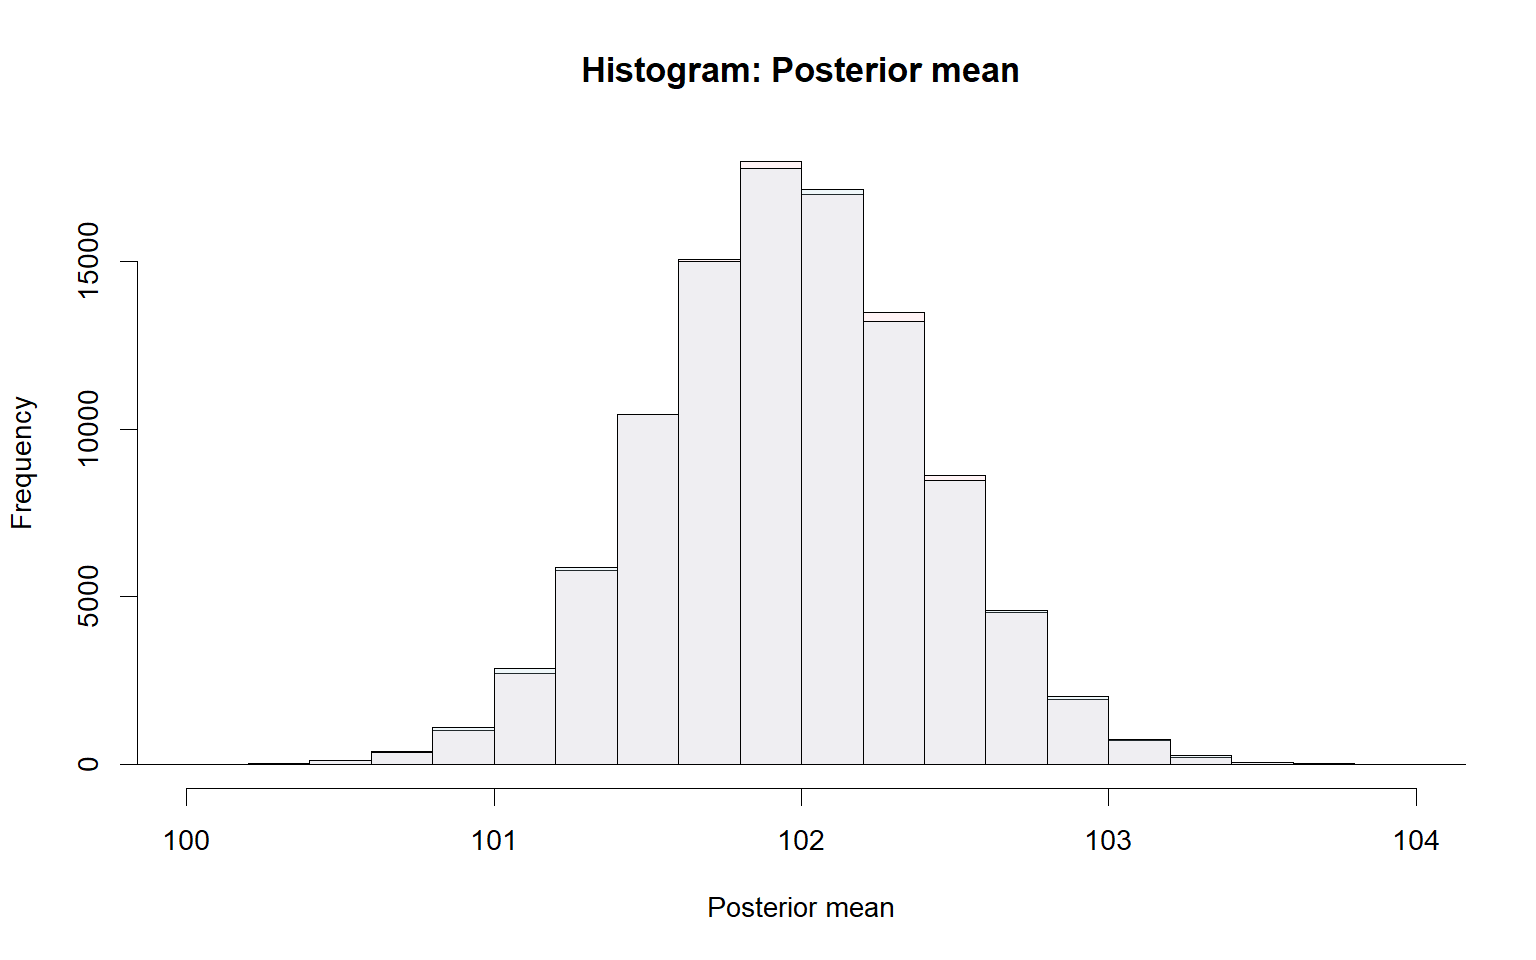
\includegraphics[width=340pt, height=200pt]{Chapters/chapter4/figures/conditionalVSmarginal.png}
	%%\centerline{\epsfig{/Chapters/chapter1/figures/cat.eps,width=.8\textheight,height=.4\textwidth}}
	\caption[List of figure caption goes here]{Histogram using the posterior conditional distribution and the posterior marginal distribution}\label{fig42}
\end{figure}


We have that the 95\% credible interval is (101.08, 102.84), and the probability of having a value greater than 103 is 1.09\%. 

%\item In the optimal tangency portfolio example, what are the equations for $\mu_{T+\kappa}=\mu_{n}$ and ${\bf\Sigma}_{T+\kappa}$? Use these equations to find the optimal weights six periods ahead using the tech stocks. 

%{\textbf{Answer}} 

\item \textbf{Demand of electricity example continues}

Set $c_0$ such that maximizes the marginal likelihood in the specifications with and without electricity price in the example of demand of electricity (empirical Bayes). Then, calculate the Bayes factor, and conclude if there is evidence supporting the inclusion of the price of electricity in the demand equation. 

{\textbf{Answer}} 

\begin{tcolorbox}[enhanced,width=4.67in,center upper,
	fontupper=\large\bfseries,drop shadow southwest,sharp corners]
	\textit{R code. Demand of electricity}
	\begin{VF}
		\begin{lstlisting}[language=R]
rm(list = ls())
set.seed(010101)
# Electricity demand
DataUt <- read.csv("DataApplications/Utilities.csv", sep = ",", header = TRUE, fileEncoding = "latin1")
DataUtEst <- DataUt %>% 
filter(Electricity != 0)
attach(DataUtEst)
# Dependent variable: Monthly consumption (kWh) in log
Y <- log(Electricity)
N <- length(Y)
# Regressors quantity including intercept
X <- cbind(LnPriceElect, IndSocio1, IndSocio2, Altitude, Nrooms, HouseholdMem, Children, Lnincome, 1)
# Regressor without price
Xnew <- cbind(IndSocio1, IndSocio2, Altitude, Nrooms, HouseholdMem, Children, Lnincome, 1)
# Log marginal function (multiply by -1 due to minimization)
LogMarLikLM <- function(X, c0){
	k <- dim(X)[2]
	N <- dim(X)[1]	
	# Hyperparameters
	B0 <- c0*diag(k)
	b0 <- rep(0, k)
	# Posterior parameters
	bhat <- solve(t(X)%*%X)%*%t(X)%*%Y
	# Force this matrix to be symmetric
	Bn <- as.matrix(Matrix::forceSymmetric(solve(solve(B0) + t(X)%*%X))) 
	bn <- Bn%*%(solve(B0)%*%b0 + t(X)%*%X%*%bhat)
	dn <- as.numeric(d0 + t(Y)%*%Y+t(b0)%*%solve(B0)%*%b0-t(bn)%*%solve(Bn)%*%bn)
	an <- a0 + N
	# Log marginal likelihood
	logpy <- (N/2)*log(1/pi)+(a0/2)*log(d0)-(an/2)*log(dn) + 0.5*log(det(Bn)/det(B0)) + lgamma(an/2)-lgamma(a0/2)
	return(-logpy)
}
# Hyperparameters
d0 <- 0.001/2
a0 <- 0.001/2
# Empirical Bayes: Obtain c0 maximizing the log marginal likelihood
c0 <- 1000 
EB <- optim(c0, fn = LogMarLikLM, method = "Brent", lower = 0.0001, upper = 10^6, X = X)
EBnew <- optim(c0, fn = LogMarLikLM, method = "Brent", lower = 0.0001, upper = 10^6, X = Xnew)
# Change of order to take into account the -1 in the LogMarLikLM function
BFEM <- exp(EBnew$value - EB$value) 
BFEM
71897938
\end{lstlisting}
	\end{VF}
\end{tcolorbox} 

The Bayes factor based on the empirical Bayes of the model with electricity price versus the model without electricity price is equal to 71897938, this gives very strong evidence to include the price in the specification.
 
\item \textbf{Utility demand}

Use the file \textit{Utilities.csv} to estimate a multivariate linear regression model where $\mathbf{Y}_i=\left[\log(\text{electricity}_i) \ \log(\text{water}_i) \ \log(\text{gas}_i)\right]$ as function of $\log(\text{electricity price}_i)$, $\log(\text{water price}_i)$, $\log(\text{gas price}_i)$, $\text{IndSocio1}_i$, $\text{IndSocio2}_i$, $\text{Altitude}_i$, $\text{Nrooms}_i$, $\text{HouseholdMem}_i$, $\text{Children}_i$, and $\log(\text{Income}_i)$, where electricity, water and gas are monthly consumption of electricity (kWh), water (m$^3$) and gas (m$^3$), and other definitions are given in the Example of Section 4.3. Omit households that do not consume any of the utilities in this exercise. 

Set a non-informative prior framework, $\mathbf{B}_0=\left[0\right]_{11\times 3}$, $\mathbf{V}_0=1000 \mathbf{I}_{11}$, $\mathbf{\Psi}_0=1000 \mathbf{I}_{3}$ and $\alpha_0=3$, where we have $K=11$ (regressors plus intercept) and $M=3$ (equations) in this exercise.

\begin{enumerate}
	\item Find the posterior mean estimates and the highest posterior density intervals at 95\% of $\mathbf{B}$ and $\mathbf{\Sigma}$. Use the marginal distribution and the conditional distribution to obtain the posterior estimates of  $\mathbf{B}$, and compare the results.
	\item Find the Bayes factor comparing the baseline model in this exercise with the same specification but using the income in dollars. Now, calculate the Bayes factor using the income in thousand dollars. Is there any difference?
	\item Find the predictive distribution for the monthly demand of electricity, water and gas in the baseline specification of a household located in the lowest socioeconomic condition in a municipality located below 1000 meters above the sea level, 2 rooms, 3 members with children, a monthly income equal to USD 500, an electricity price equal to USD/kWh 0.15, a water price equal to USD/M$^3$ 0.70, and a gas price equal to USD/M$^3$ 0.75. 
\end{enumerate}   

{\textbf{Answer}} 

We see that the posterior estimates of the location parameters based on the marginal distribution and the conditional distribution are very similar (conditional on $\mathbf{\Sigma}$). This is important as many times there is no analytical solutions in well-known forms of marginal posterior distributions, and consequently, we should get draws of the posterior distributions based on conditional distributions of block of parameters (See Chapter \ref{chap5}).

We find that the Bayes factor of the baseline model ($\log(\text{Income})$) versus the two alternative models using income in dollars and thousand dollars are 108925764 and 0.1089261. The former gives strong evidence in favor of the baseline model, whereas the latter gives positive evidence for the model using the income in thousand dollars. This result despite that the location coefficients are the same in the two alternative specifications, except for the change in scale of the coefficients associated with income. This example shows that Bayes factors are sensitive to units of measure, and consequently, it is relevant to think carefully about the priors when performing hypothesis testing using a Bayesian framework. Observe that a nice feature in Bayesian inference is that we followed the same conceptual framework (Bayes factor) in the previous exercise and this exercise. In one hand, the previous exercise is an example of nested models, that is, one model is a restricted version of a more general model. On the other hand, this exercise is an example of non-nested models. This is not the case in the Frequentist approach. The statistical framework is not the same when testing nested and non-nested models.

\begin{tcolorbox}[enhanced,width=4.67in,center upper,
	fontupper=\large\bfseries,drop shadow southwest,sharp corners]
	\textit{R code. Utilities demand: Multivariate regression, posterior inference}
	\begin{VF}
		\begin{lstlisting}[language=R]
rm(list = ls())
set.seed(010101)
library(dplyr)
# Electricity demand
DataUt <- read.csv("DataApplications/Utilities.csv", sep = ",", header = TRUE, fileEncoding = "latin1")
DataUtEst <- DataUt %>%  
filter(Electricity != 0 & Water !=0 & Gas != 0)
attach(DataUtEst)
Y <- cbind(log(Electricity), log(Water), log(Gas))
X <- cbind(LnPriceElect, LnPriceWater, LnPriceGas, IndSocio1, IndSocio2, Altitude, Nrooms, HouseholdMem, Children, Lnincome, 1)
M <- dim(Y)[2]
K <- dim(X)[2]
N <- dim(Y)[1]
# Hyperparameters
B0 <- matrix(0, K, M)
c0 <- 1000
V0 <- c0*diag(K)
Psi0 <- c0*diag(M)
a0 <- M
# Posterior parameters
Bhat <- solve(t(X)%*%X)%*%t(X)%*%Y 
S <- t(Y - X%*%Bhat)%*%(Y - X%*%Bhat)
Vn <- solve(solve(V0) + t(X)%*%X) 
Bn <- Vn%*%(solve(V0)%*%B0 + t(X)%*%X%*%Bhat)
Psin <- Psi0 + S + t(B0)%*%solve(V0)%*%B0 + t(Bhat)%*%t(X)%*%X%*%Bhat - t(Bn)%*%solve(Vn)%*%Bn
an <- a0 + N
#Posterior draws
s <- 10000 #Number of posterior draws
SIGs <- replicate(s, LaplacesDemon::rinvwishart(an, Psin))
BsCond <- sapply(1:s, function(s) {MixMatrix::rmatrixnorm(n = 1, mean=Bn, U = Vn,V = SIGs[,,s])})
summary(coda::mcmc(t(BsCond)))
Bs <- sapply(1:s, function(s) {MixMatrix::rmatrixt(n = 1, mean=Bn, U = Vn,V = Psin, df = an + 1 - M)})
summary(coda::mcmc(t(Bs)))
SIGMs <- t(sapply(1:s, function(l) {gdata::lowerTriangle(SIGs[,,l], diag=TRUE, byrow=FALSE)}))
summary(coda::mcmc(SIGMs))
hdiBs <- HDInterval::hdi(t(BsCond), credMass = 0.95) # Highest posterior density credible interval
hdiBs
hdiSIG <- HDInterval::hdi(SIGMs, credMass = 0.95) # Highest posterior density credible interval
hdiSIG
		\end{lstlisting}
	\end{VF}
\end{tcolorbox} 

\begin{tcolorbox}[enhanced,width=4.67in,center upper,
	fontupper=\large\bfseries,drop shadow southwest,sharp corners]
	\textit{R code. Utilities demand: Multivariate regression, Bayes factors}
	\begin{VF}
		\begin{lstlisting}[language=R]
# Log marginal function (multiply by -1 due to minimization)
LogMarLikLM <- function(X, c0){
	c10 <- c0[1]; c20 <- c0[2]
	k <- dim(X)[2]
	N <- dim(X)[1]
	# Hyperparameters
	V0 <- c10*diag(K)
	Psi0 <- c20*diag(M)
	# Posterior parameters
	Bhat <- solve(t(X)%*%X)%*%t(X)%*%Y 
	S <- t(Y - X%*%Bhat)%*%(Y - X%*%Bhat)
	Vn <- solve(solve(V0) + t(X)%*%X) 
	Bn <- Vn%*%(solve(V0)%*%B0 + t(X)%*%X%*%Bhat)
	Psin <- Psi0 + S + t(B0)%*%solve(V0)%*%B0 + t(Bhat)%*%t(X)%*%X%*%Bhat - t(Bn)%*%solve(Vn)%*%Bn
	# Log marginal likelihood
	logpy <- (N*M/2)*log(1/pi)+(a0/2)*log(det(Psi0)) - (an/2)*log(det(Psin)) + (M/2)*(log(det(Vn)) - log(det(V0))) + lgamma(an/2)-lgamma(a0/2)
	return(-logpy)
}
c0 <- rep(1000, 2)
LogML <- LogMarLikLM(X=X, c0 = c0)
# Using income in dollars as regressor
Xnew <- cbind(LnPriceElect, LnPriceWater, LnPriceGas, IndSocio1, IndSocio2, Altitude, Nrooms, HouseholdMem, Children, exp(Lnincome), 1)
LogMLnew <- LogMarLikLM(X=Xnew, c0 = c0)
# Bayes factor
BF12 <- exp(LogMLnew - LogML)
BF12
# Using income in thousand dollars as regressor
XnewT <- cbind(LnPriceElect, LnPriceWater, LnPriceGas, IndSocio1, IndSocio2, Altitude, Nrooms, HouseholdMem, Children, exp(Lnincome)/1000, 1)
LogMLnewT <- LogMarLikLM(X=XnewT, c0 = c0)
# Bayes factor
BF13 <- exp(LogMLnewT - LogML)
BF13
		\end{lstlisting}
	\end{VF}
\end{tcolorbox} 

\begin{tcolorbox}[enhanced,width=4.67in,center upper,
	fontupper=\large\bfseries,drop shadow southwest,sharp corners]
	\textit{R code. Utilities demand: Multivariate regression, predictive distribution}
	\begin{VF}
		\begin{lstlisting}[language=R]
# Predictive distribution
Xpred <- c(log(0.15), log(0.70), log(0.75), 1, 0, 0, 2, 3, 1, log(500), 1)
Mean <- Xpred%*%Bn
Hn <- 1+t(Xpred)%*%Vn%*%Xpred
UtilDemand <- exp(replicate(s, MixMatrix::rmatrixt(n = 1, mean=Mean, U = Hn, V = Psin, df = an + 1 - M)))
ElePred <- UtilDemand[1,1,]
WatPred <- UtilDemand[1,2,]
GasPred <- UtilDemand[1,3,]
data <- data.frame(cbind(ElePred, WatPred, GasPred)) #Data frame
annotations1 <- data.frame(
x = round(quantile(data$ElePred, c(0.025, 0.5, 0.975)),1),
y = c(600, 1000, 600),
label = c("2.5%:", "50%:", "97.5%:")
)
annotations2 <- data.frame(
x = round(quantile(data$WatPred, c(0.025, 0.5, 0.975)),1),
y = c(600, 1000, 600),
label = c("2.5%:", "50%:", "97.5%:")
)
annotations3 <- data.frame(
x = round(quantile(data$GasPred, c(0.025, 0.5, 0.975)),1),
y = c(600, 1000, 600),
label = c("2.5%:", "50%:", "97.5%:")
)
require(ggplot2) # Cool figures
require(ggpubr) # Multiple figures in one page
require(latex2exp) # LaTeX equations in figures
fig1 <- ggplot(data = data, aes(ElePred)) + geom_histogram(bins = 40, color = "#000000", fill = "#0099F8") + 	xlab("kWh") + ylab("Frequency") +	ggtitle("Electricity") + xlim(0, 1050) + geom_text(data = annotations1, aes(x = x, y = y, label = paste(label, x)), size = 3, fontface = "bold")
fig2 <- ggplot(data = data, aes(WatPred)) + geom_histogram(bins = 40, color = "#000000", fill = "#0099F8") + 	xlab(TeX("$M^3$")) + ylab("Frequency") +	ggtitle("Water") + xlim(0, 100) + geom_text(data = annotations2, aes(x = x, y = y, label = paste(label, x)), size = 3, fontface = "bold")
fig3 <- ggplot(data = data, aes(GasPred)) + geom_histogram(bins = 40, color = "#000000", fill = "#0099F8") + 	xlab(TeX("$M^3$")) + ylab("Frequency") +	ggtitle("Gas") + xlim(0, 80) + geom_text(data = annotations3, aes(x = x, y = y, label = paste(label, x)), size = 3, fontface = "bold")
		\end{lstlisting}
	\end{VF}
\end{tcolorbox} 


Figures \ref{fig13}, \ref{fig14} and \ref{fig15} show the marginal predictive distributions of electricity, water and gas for the reference household. The median predictive values are kWh 168.8, M$^3$ 12.3 and M$^3$ 10.1, respectively. In addition, the 95\% credible intervals are (27.7, 1028.9), (1.5, 98.7) and (1.5, 67.5) for electricity, water and gas.  

\begin{figure}[!h]
	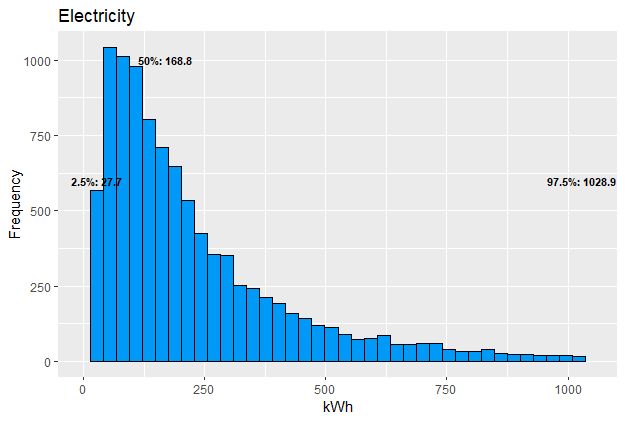
\includegraphics[width=340pt, height=200pt]{Chapters/chapter4/figures/ElectMulti.png}
	%%\centerline{\epsfig{/Chapters/chapter1/figures/cat.eps,width=.8\textheight,height=.4\textwidth}}
	\caption[List of figure caption goes here]{Histogram using the posterior predictive distribution of electricity demand}\label{fig13}
\end{figure}

\begin{figure}[!h]
	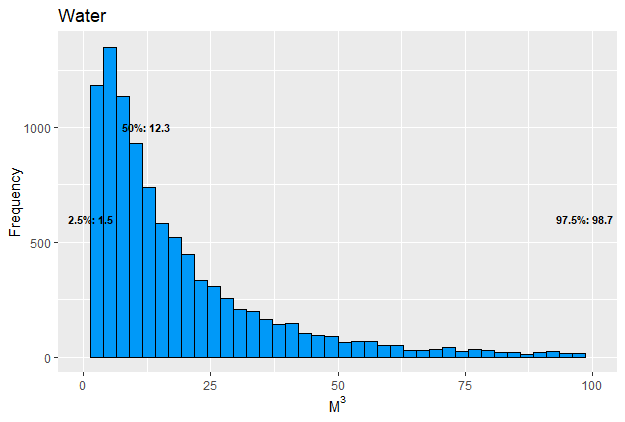
\includegraphics[width=340pt, height=200pt]{Chapters/chapter4/figures/WaterMulti.png}
	%%\centerline{\epsfig{/Chapters/chapter1/figures/cat.eps,width=.8\textheight,height=.4\textwidth}}
	\caption[List of figure caption goes here]{Histogram using the posterior predictive distribution of water demand}\label{fig14}
\end{figure}  

\begin{figure}[!h]
	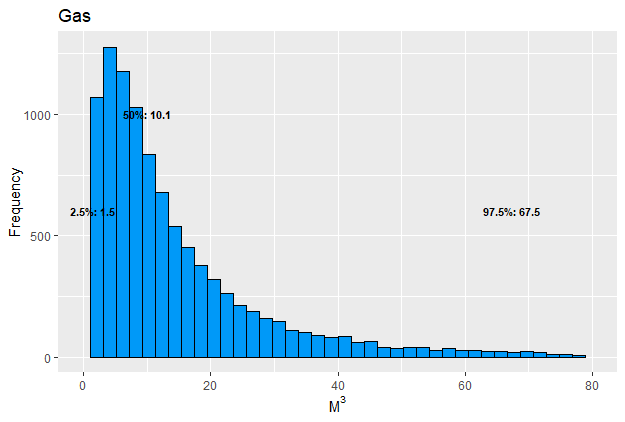
\includegraphics[width=340pt, height=200pt]{Chapters/chapter4/figures/GasMulti.png}
	%%\centerline{\epsfig{/Chapters/chapter1/figures/cat.eps,width=.8\textheight,height=.4\textwidth}}
	\caption[List of figure caption goes here]{Histogram using the posterior predictive distribution of gas demand}\label{fig15}
\end{figure}    
\end{enumerate}



